%
% problemstellung.tex -- Beispiel-File für die Beschreibung des Problems
%
% (c) 2020 Prof Dr Andreas Müller, Hochschule Rapperswil
%
\section{Potenzreihen
\label{pade:section:Potenzreihen}}
\rhead{Potenzreihen}
In der Analysis kann eine Funktion mit einer Taylorreihe um eine Stelle $x_{0}$ durch eine Potenzreihe dargestellt werden. 
Diese Potenzreihen werden um einen vorgegebene Stelle $x_{0}$ als eine unendliche Summe 
\begin{equation}
f(x)=\sum_{n=0}^{\infty} a_{n} (x-x_{0})^{n} 
\end{equation}
gebildet.
Für viele Funktionen sind die dazugehörigen Potenzreihen schon bekannt. 
Funktionen welche durch eine Potenzreihe dargestellt werden können auch analytische Funktionen genannt werden.
Es gibt verschiedene Methoden um eine Potenzreihe einer Funktion zu erhalten. 
Bei analytischen Funktionen sind die Potenzreihen schon bekannt und können etwa durch Differentialgleichungen oder eine andere Reihenentwicklungsmethode hergeleitet werden.
Wie die Herleitung mit einer Potenzreihe mit einer Differentialgleichung wird in dem Abschnitt \ref{pade:section:Bsp_Potenzreihen} gezeigt.

\subsection{Beispiel Potenzreihen
\label{pade:section:Bsp_Potenzreihen}}
Aus der Exponentialfunktion
\begin{equation*}
e^{x}
=
\sum_{n=0}^{\infty} \frac{x^{n}}{n !}
=
\frac{x^{0}}{0 !}+\frac{x^{1}}{1 !}+\frac{x^{2}}{2 !}+\frac{x^{3}}{3 !}+\cdots 
\end{equation*}
für alle $x \in \mathbb{R}$ d.h., der Konvergenzradius der Potenzreihe ist unendlich, kann durch Gebrauch von Euler sogleich die Potenzreihe für den Sinus und Kosinus ermittelt werden
\begin{align*}
e^{ix}
&=
\sum_{n=0}^{\infty} \frac{(ix)^{n}}{n !}
=
\frac{(ix)^{0}}{0 !}+\frac{(ix)^{1}}{1 !}+\frac{(ix)^{2}}{2 !}+\frac{(ix)^{3}}{3 !}+\cdots
\\
&=
\left(1-\frac{x^{2}}{2 !}+\frac{x^{4}}{4 !}-\ldots\right)+\mathrm{i} \cdot\left(x-\frac{x^{3}}{3 !}+\frac{x^{5}}{5 !}-\ldots\right)
\\
&=
\cos(x)+i\cdot \sin(x).
\end{align*}
Wobei die Sinusfunktion 
\begin{equation*}
\sin (x)=\sum_{n=0}^{\infty}(-1)^{n} \frac{x^{2 n+1}}{(2 n+1) !}=\frac{x}{1 !}-\frac{x^{3}}{3 !}+\frac{x^{5}}{5 !} \mp \cdots
\end{equation*}
und die Kosinusfunktion 
\begin{equation*}
\cos (x)=\sum_{n=0}^{\infty}(-1)^{n} \frac{x^{2 n}}{(2 n) !}=\frac{x^{0}}{0 !}-\frac{x^{2}}{2 !}+\frac{x^{4}}{4 !} \mp \cdots
\end{equation*}



\section{Das Taylorreihen Problem
\label{pade:Taylorfehler}}
Für praktischen Berechnungen von Modellen in der Physik, Ingenieurwissenschaften und weiteren Feldern wird die Taylorreihe schon früh im Studium als ein nützliches Hilfsmittel gelehrt.
Die klassische Antwort auf eine Taylorreihe welche konvergiert ist, dass sie den Wert einer Funktion welche beliebig oft Abgeleitet werden kann definiert. 
In der Praxis wird die Funktion jedoch nur mit immer längeren Polynomen approximiert.
Diese Methode kann bei praktischen Problemen auch einen sehr unerwünschte und limitierenden Effekt haben. 
Schauen wir das Beispiel 
\begin{equation*}
f(x)
=
(\frac{1+2x}{1+x})^{\frac{1}{2}}
\approx
1+\frac{1}{2}x - \frac{5}{8}x^2+\frac{13}{16}x^3 -\frac{141}{128}x^4 +\frac{399}{256}x^5 - \frac{2353}{1024}x^6 + \frac{7205}{2048}x^7 \mp \cdots
\end{equation*}
an. 
Die originale Funktion $f(x)$ ist eine zwische $0<x<\infty$ einfache und stetige Funktion welche sich von $1$ zu $\sqrt{2}$ bewegt.
Die Dazugehörige Taylorreihe ist jedoch nicht in der Lage bei einem Wert von $x>\frac{1}{2}$ zu konvergieren. 
Das verhalten der original Funktion und dessen Taylorreihe ist in dem Graphen \ref{pade:prob1} ersichtlich. 


\begin{figure}[ht]
	\centering
	\subfigure[Plot von $f(x)$ und Taylorreihe 7. Ordnung\label{pade:prob1}]{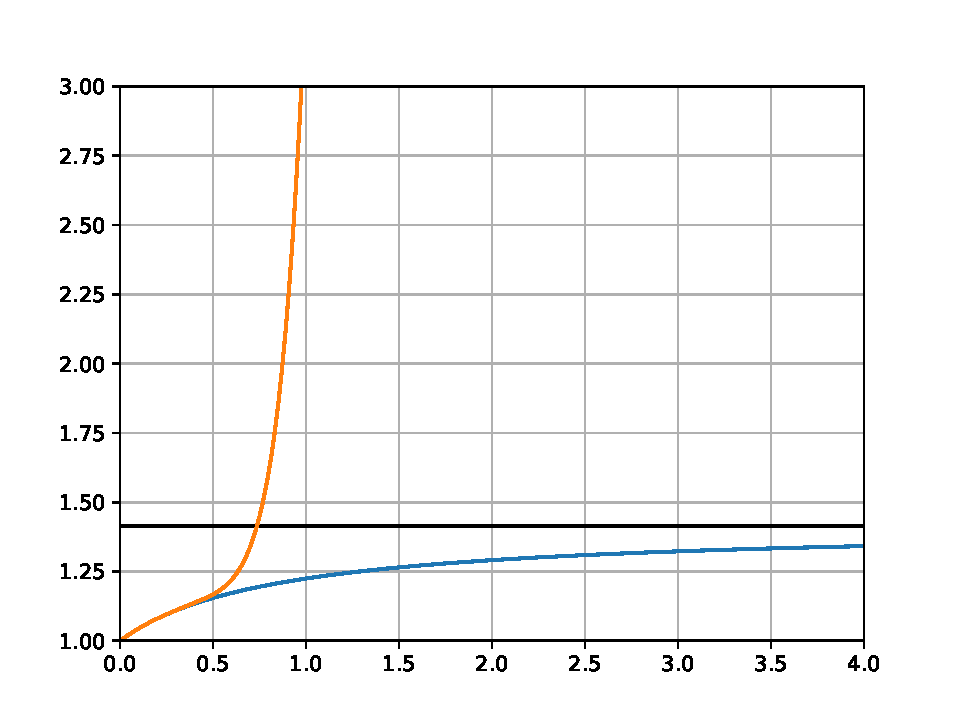
\includegraphics[width=0.45\linewidth]{./papers/pade/python/bilder/taylorProb1.pdf}}
	\subfigure[Fehler zwischen der Funktion und der Approximation\label{pade:prob2}]{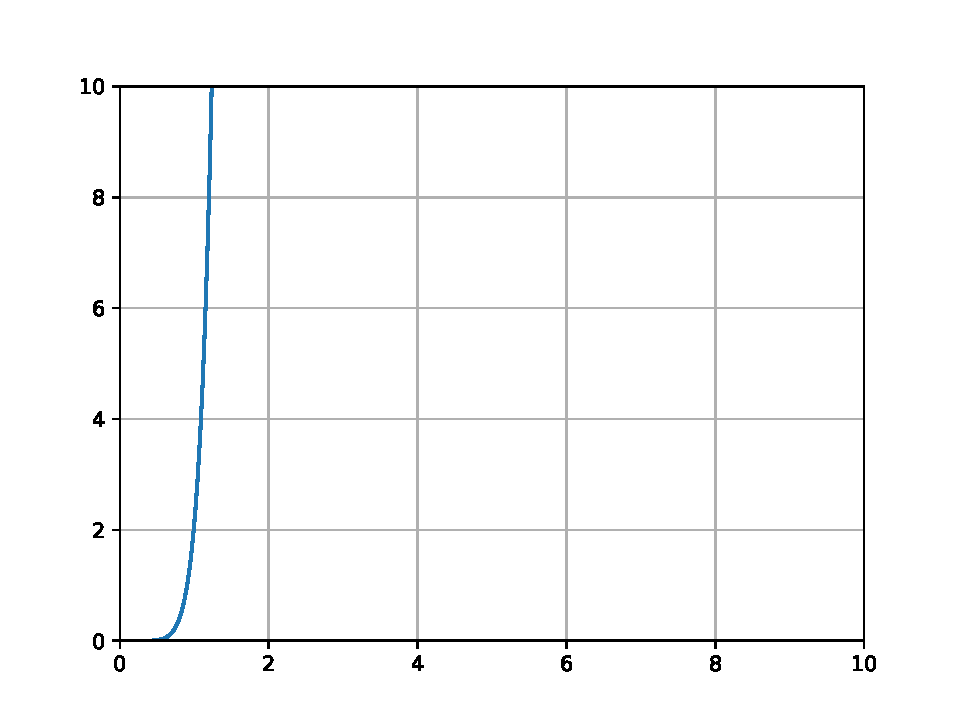
\includegraphics[width=0.45\linewidth]{./papers/pade/python/bilder/taylorProb3.pdf}}
	\subfigure[Plot von $f(x)$ und Padeapproximation 3. Ordnung\label{pade:prob3}]{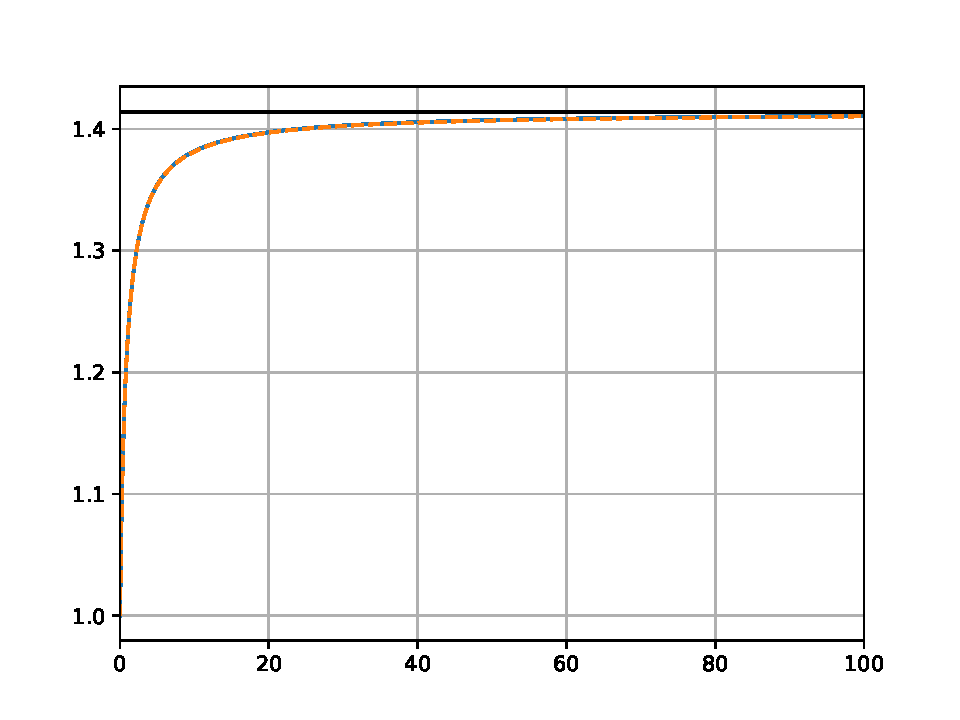
\includegraphics[width=0.45\linewidth]{./papers/pade/python/bilder/taylorProb2.pdf}}
	\subfigure[Fehler zwischen der Funktion und der  Padeapproximation\label{pade:prob4}]{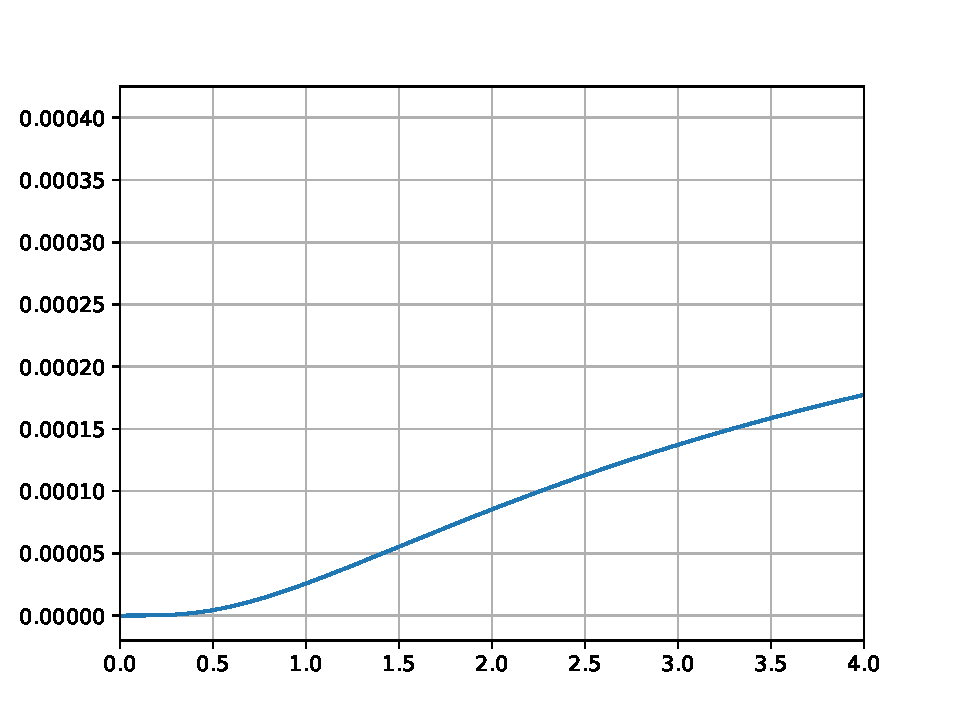
\includegraphics[width=0.45\linewidth]{./papers/pade/python/bilder/taylorProb4.pdf}}
	\caption{Visualisierung von der Funktion $f(x)$ und dessen Approximation\label{pade:prob}}
\end{figure}



